\documentclass[../main.tex]{subfiles}

\begin{document}

\begin{problem}
In the proof of finiteness theorem, we have $\left \| s \right \|_U\leq A\left \| s \right \|_V$ \\
where $A:=\displaystyle\max_{i,j}\sup_{x\in U_i\cap U_j}\left \| g_{ij}(x) \right \|$, $\forall s\in H^0(X,L)$ \\
$\forall s\in H^0(X,L), \mathrm{ord}_{a_i}s_i\geq l$, $\left \| s \right \|_U\leq A\left \| s \right \|_V\leq 2^{-l}A\left \| s \right \|_U$, thus $$H^0(X,L)\rightarrow \displaystyle\bigoplus_{i=1}^{N}\mathbb{C}\otimes\left(\mathcal{O}_{a_i}/m_i^{l}\right),\,s\mapsto\displaystyle\bigoplus_{i=1}^{N}\left(s_i\,\mathrm{mod}\,z_i^l\right)$$
is injective if $2^l>A$, thus $\dim H^0(X,L)\leq Nl=:C$ \\
But now we have $\left \| s \right \|_U\leq A^k\left \| s \right \|_V$, $\forall s\in H^0(X,L)$ \\
since $|s_i(x)|=|g_{ij}(x)^ks_j(x)|\leq \left \| g_{ij}(x) \right \|^k|s_j(x)|$ \\
$\forall s\in H^0(X,L^k), \mathrm{ord}_{a_i}s_i\geq kl$, $\left \| s \right \|_U\leq A\left \| s \right \|_V\leq 2^{-kl}A\left \| s \right \|_U$, thus $$H^0(X,L^k)\rightarrow \displaystyle\bigoplus_{i=1}^{N}\mathbb{C}\otimes\left(\mathcal{O}_{a_i}/m_i^{kl}\right),\,s\mapsto\displaystyle\bigoplus_{i=1}^{N}\left(s_i\,\mathrm{mod}\,z_i^{kl}\right)$$
is injective if $2^l>A\Rightarrow 2^{kl}>A^k$, thus $\dim H^0(X,L^k)\leq Nkl=:Ck$
\end{problem}

\begin{problem}
Suppose there are more than $2k$ fixed points of $\sigma$, then consider $f-f\circ\sigma^{-1}: X\rightarrow\mathbb{P}^1$ is holomorphic on $X\setminus\{a,\sigma^{-1}(a)\}$ with at least $2k+1$ zeros and with poles of order $k$ at $a, \sigma^{-1}(a)$, but it should have as many poles as zeros which is a contradiction
\end{problem}

\begin{problem}
The genus $g$ of $\mathbb{P}^1$ is $0$ \par
If $\deg D<0$, then $\forall f\in H^0(\mathbb{P}^1,\mathcal{O}_D)\subseteq\mathcal{M}(\mathbb{P}^1)$, then $0=\deg\mathrm{div}(f)\geq \deg(-D)=-\deg D>0$ which is impossible, hence $\dim H^0(\mathbb{P}^1,\mathcal{O}_D)=0$ and $\dim H^1(\mathbb{P}^1,\mathcal{O}_D)=-1-\deg D$ \par
If $\deg D\geq 0$, since from the long exact sequence we already knew that $H^1(\mathbb{P}^1,\mathcal{O}_D')\rightarrow H^0(\mathbb{P}^1,\mathcal{O}_D)\rightarrow 0$ is exact if $D'\leq D$, and we can always find a $D'$ such that $D'\leq D$ and $\deg D'<0$, then $0=\dim H^1(\mathbb{P}^1,\mathcal{O}_D')\geq \dim H^1(\mathbb{P}^1,\mathcal{O}_D)\geq 0$, thus $\dim H^1(\mathbb{P}^1,\mathcal{O}_D)=0$ and $\dim H^0(\mathbb{P}^1,\mathcal{O}_D)=1+\deg D$ \par
Therefore, we have \par
\[
\begin{aligned}
&\dim H^0(\mathbb{P}^1,\mathcal{O}_D)=\max\left(0,1+\deg D\right) \\
&\dim H^1(\mathbb{P}^1,\mathcal{O}_D)=\max\left(0,-1-\deg D\right)
\end{aligned}
\]
\end{problem}

\begin{problem}
\begin{center}
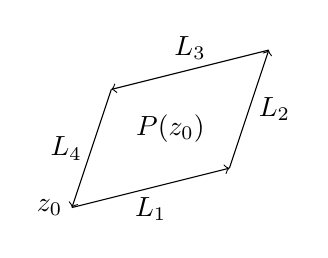
\begin{tikzpicture}[scale=0.5]
\node[below,left]at (0, 0){$z_0$};
\draw[->] (0,0)--(4,1);
\node[below]at (2, 0.5){$L_1$};
\draw[->] (4,1)--(5,4);
\node[right]at (4.5, 2.5){$L_2$};
\draw[->] (5,4)--(1,3);
\node[above]at (3, 3.5){$L_3$};
\draw[->] (1,3)--(0,0);
\node[left]at (0.5, 1.5){$L_4$};
\node at (2.5, 2){$P(z_0)$};
\end{tikzpicture}
\end{center}
\textbf{a.} \par
Since $f$ is elliptic, $\displaystyle\int_{L_1}f(z)dz=-\int_{L_3}f(z)dz,\int_{L_2}f(z)dz=-\int_{L_4}f(z)dz$, thus $\displaystyle\int_{\partial P(z_0)}f(z)dz=\int_{L_1}f(z)dz+\int_{L_2}f(z)dz+\int_{L_3}f(z)dz+\int_{L_4}f(z)dz=0$ \par
\textbf{b.} \par
As the same reason in (a), we have $\displaystyle\dfrac{1}{2\pi i}\int_{\partial P(z_0)}\dfrac{f'(z)}{f(z)}dz=0$, by argument principle, we know in the interior of $P(z_0)$, there are as many zeros as poles, counted multiplicities \par
\end{problem}

\begin{problem}
Consider $\displaystyle\dfrac{1}{2\pi i}\int_{\partial P(z_0)}\dfrac{zf'(z)}{f(z)}dz=\sum_{j=1}^n(z_j-w_j)$ \par
On the other hand, 
\[
\begin{aligned}
&-\dfrac{1}{2\pi i}\int_{L_3}\dfrac{zf'(z)}{f(z)}dz=\dfrac{1}{2\pi i}\int_{L_1}\dfrac{(z+\omega_2)f'(z)}{f(z)}dz \\
&\dfrac{1}{2\pi i}\int_{L_2}\dfrac{zf'(z)}{f(z)}dz=-\dfrac{1}{2\pi i}\int_{L_4}\dfrac{(z+\omega_1)f'(z)}{f(z)}dz
\end{aligned}
\]
Thus
\[
\dfrac{1}{2\pi i}\int_{\partial P(z_0)}\dfrac{zf'(z)}{f(z)}dz
=\dfrac{1}{2\pi i}\left(\int_{L_1}+\int_{L_2}+\int_{L_3}+\int_{L_4}\right)\dfrac{zf'(z)}{f(z)}dz
=-\dfrac{\omega_1}{2\pi i}\int_{L_4}\dfrac{f'(z)}{f(z)}dz-\dfrac{\omega_2}{2\pi i}\int_{L_1}\dfrac{f'(z)}{f(z)}dz
\]
Hence we only need to show $\displaystyle\dfrac{1}{2\pi i}\int_{L_1}\dfrac{f'(z)}{f(z)}dz,\dfrac{1}{2\pi i}\int_{L_4}\dfrac{f'(z)}{f(z)}dz\in\mathbb{Z}$, but
$$\dfrac{1}{2\pi i}\int_{L_1}\dfrac{f'(z)}{f(z)}dz=\dfrac{1}{2\pi i}\int_{L_1}\dfrac{d(f(z))}{f(z)}=\dfrac{1}{2\pi i}\int_{f(L_1)}\dfrac{dz}{z}=k$$
For some $k\in\mathbb{Z}$
\end{problem}

\end{document}